\subsection{Impact: Thread Count}\label{sec:dspmv-threadscaling}

\begin{figure}[H]
	\begin{centering}
		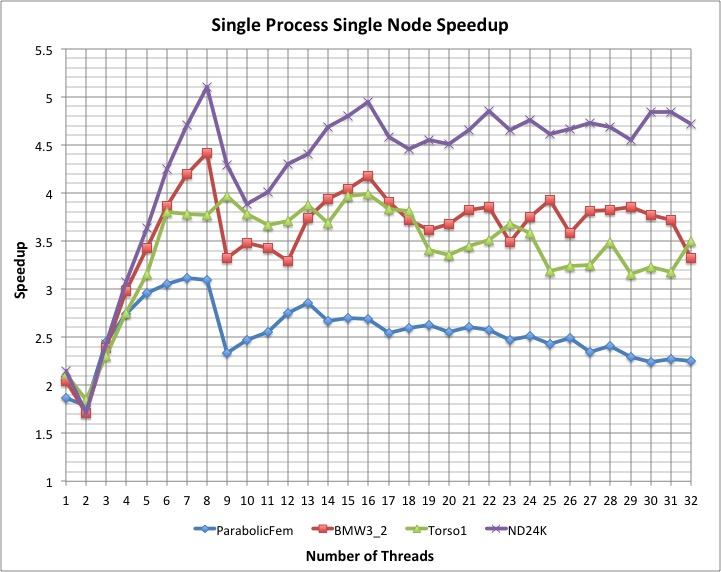
\includegraphics[scale=0.25]{figures/single_node_speedup.jpg}
		\caption{Single Node Speedup}
		\label{fig:spmv-page-singlenode}
\end{centering}
\end{figure}

Where computation is bound by memory references and cache hits capitalizing upon multi-core utilization can greatly increase performance \cite{blelloch2008provably}. In hybrid codes optimizing performance exhibited from a individual node is essential for overall execution. Figure \ref{fig:spmv-page-singlenode} illustrates the impact of increasing thread count locally on a single node due to the increased memory access as the socket cores become saturated with work. A peak can be seen near 8 threads with another visible peak at 16. 

Once all cores on a single processor are assigned a thread that chips memory bandwidth as been fully allocated thereby achieving the maximum on chip memory bandwidth. Beyond 8 threads an increase in overhead from the distribution of work amongst the disjoint memory profiles on each chip degrades performance until total memory bandwidth allocation overcomes this overhead. Over subscription of node sockets/cores produces stagnation and declines in speedup across all matrices examined. It is worth noting that the code generated for these experiments made no effort to control thread core or socket affinity, therefore it is highly likely that scheduling in an oversubscribed node is a cause for declining performance. 